
\documentclass[11pt,compress,t,notes=noshow]{beamer}

\usepackage[english]{babel}
\usepackage{dsfont}
\newcommand\bmmax{2}
\usepackage{bm}
\usepackage{bbm}
\usepackage{verbatim}
\usepackage{amsmath}
\usepackage{amsfonts}
\usepackage{csquotes}
\usepackage{multirow}
\usepackage{longtable}
\usepackage{enumerate}
\usepackage[absolute,overlay]{textpos}
\usepackage{psfrag}
\usepackage{algorithm}
\usepackage{algorithmicx}
\usepackage{algpseudocode}
\usepackage{eqnarray}
\usepackage{multimedia}
\usepackage{media9}
\usepackage{arydshln}
\usepackage{tabularx}
\usepackage{placeins}
\usepackage{tikz}
\usepackage{setspace}
\usepackage{wrapfig}
\usepackage{tcolorbox}
\usepackage[export]{adjustbox}
\usepackage{siunitx}
\usetikzlibrary{shapes,arrows,automata,positioning,calc}
\tikzset{
  %Define standard arrow tip
  >=stealth',
  %Define style for boxes
  punkt/.style={
    rectangle,
    rounded corners,
    draw=black, very thick,
    text width=6.5em,
    minimum height=2em,
    text centered},
  % Define arrow style
  pil/.style={
    ->,
    thick,
    shorten <=2pt,
    shorten >=2pt,}
}
\usepackage{subfig}

%new environments

\newenvironment{vbframe}  %frame with breaks and verbatim
{
 \begin{frame}[containsverbatim,allowframebreaks]
}
{
\end{frame}
}

\newenvironment{vframe}  %frame with verbatim without breaks (to avoid numbering one slided frames)
{
 \begin{frame}[containsverbatim]
}
{
\end{frame}
}

\newenvironment{blocki}[1]   % itemize block
{
 \begin{block}{#1}\begin{itemize}
}
{
\end{itemize}\end{block}
}

\newenvironment{fragileframe}[2]{  %fragile frame with framebreaks
\begin{frame}[allowframebreaks, fragile, environment = fragileframe]
\frametitle{#1}
#2}
{\end{frame}}


\newcommand{\myframe}[2]{  %short for frame with framebreaks
\begin{frame}[allowframebreaks]
\frametitle{#1}
#2
\end{frame}}

\newcommand{\remark}[1]{
  \textbf{Remark:} #1
}

%%%%%%%%%%%%%%%%%%%%%%%%%%%%%%%%%%%%%%%%%%%%%%%%%%%%%%%%%%%%%%%%%%%%%%%%%%%%%%%

% basic latex stuff
\newcommand{\pkg}[1]{{\fontseries{b}\selectfont #1}} %fontstyle for R packages
\newcommand{\lz}{\vspace{0.5cm}} %vertical space
\newcommand{\dlz}{\vspace{1cm}} %double vertical space
\newcommand{\oneliner}[1] % Oneliner for important statements
{\begin{block}{}\begin{center}\begin{Large}#1\end{Large}\end{center}\end{block}}


%\usetheme{lmu-lecture}
\usepackage{../style/lmu-lecture}

\let\code=\texttt
\let\proglang=\textsf

\setkeys{Gin}{width=0.9\textwidth}



\title{Deep Learning}
\author{David Rügamer}
\institute{Department of Statistics -- LMU Munich}
\date{Winter Semester 2021}

\setbeamertemplate{frametitle}{\expandafter\uppercase\expandafter\insertframetitle}

%\begin{document}
%\sloppy
%\end{document}

  
\input{../../latex-math/basic-math}
\input{../../latex-math/basic-ml}
\input{../../latex-math/ml-nn}

\newcommand{\Dsubtrain}{\mathcal{D}_{\text{subtrain}}}
\newcommand{\Dval}{\mathcal{D}_{\text{val}}}

\begin{document}

\lecturechapter{3}{Dropout}
\lecture{Deeplearning}
%%%%%%%%%%%%%%%%%%%%%%%%%%%%%%%%%%%%%%%%%%%%%%%%%%%%%%%%%%%%%%%%%%

% \begin{frame}
% \frametitle{Lecture outline}
% \tableofcontents
% \end{frame}
%%%%%%%%%%%%%%%%%%%%%%%%%%%%%%%%%%%%%%%%%%%%%%%%%%%%%%%%%%%%%%%%%%

% \section{Ensemble Methods}
% 
%   
%   \begin{vbframe}{Ensemble Methods}
% \begin{itemize}
% \item Idea: Train \textbf{several models} separately, and \textbf{average their prediction} (i.e.~perform \textbf{model averaging}).
% %$$\frac{1}{k} \sum_{i=1}^k f_k(x|\theta)$$
%   \item This improves performance on the test set, since we reduce model variance through averaging. Thus, bagging can be seen as another regularization technique. 
% \item Ensembles can be constructed in different ways, e.g.:
%   \begin{itemize}
% \item by combining completely different models (with different learning algorithms and loss functions).
% \item by \textbf{bagging}: Train the same type of model on $k$ datasets created by sampling $n$ samples (with replacement) from the original dataset.
% \end{itemize}
% \item Since training a neural network can result in different solutions (why?), it can even make sense to combine them.
% \end{itemize}
% 
% \framebreak 
% 
% \begin{figure}
% \captionsetup{font=footnotesize,labelfont=footnotesize, labelfont = bf}
% \centering
% 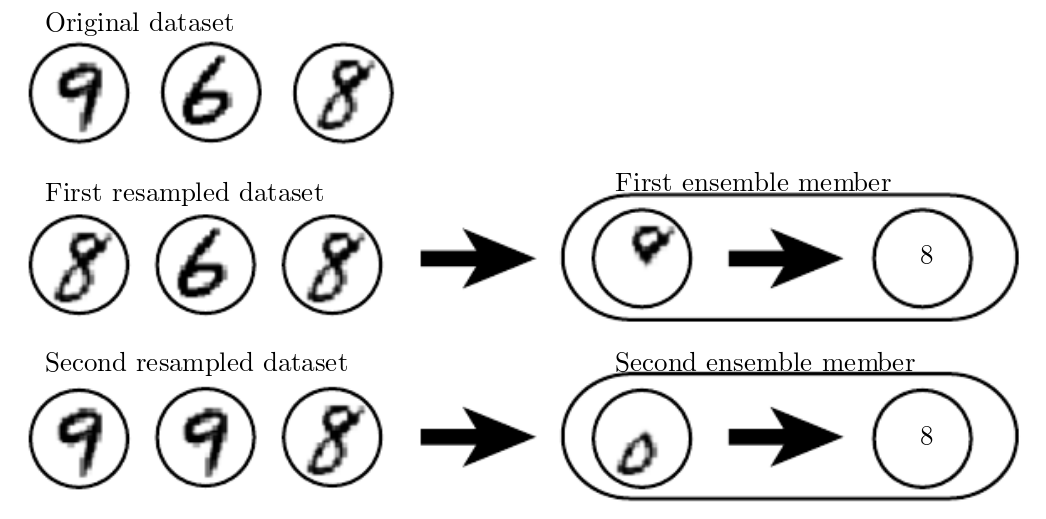
\includegraphics[width=9cm]{plots/bagging.png}
% \tiny{\\Source: Goodfellow et al. (2016), ch. 7.11}
% \caption{Cartoon depicting bagging used to train a 8 detector.
%   Top: Original training dataset; Middle: First dataset created by sampling with replacement from the training dataset. The detector learns that a loop on top of the digit corresponds to an 8; Bottom: Second dataset created by sampling with replacement. The detector learns that a loop on the bottom of the digit corresponds to an 8.
%   Both classification rules are brittle, but if we average their output, then the detector is robust. It achievs maximal confidence only when both loops of the 8 are present.}
% \end{figure}
% 
% \end{vbframe}

\section{Dropout}


\begin{vbframe}{Dropout}
\begin{itemize}
%\item{As a first approximation, dropout can be thought of as a method of making bagging practical for ensembles of very many large neural networks.}
%\item Recalling bagging, the idea is to bootstrap several models by constructing several different datasets. Afterwards the models vote on the output for test examples, which is also called model averaging.
%\item This improves the performance on the test set, since we reduce the model variance through averaging. Thus, bagging can be seen as another regularization technique. 
\item{For deep learning bagging seems impractical, since it is computationally costly to train and evaluate so many networks.}
\item Idea: Overfitting in neural networks is reduced by preventing complex
co-adaptations of neurons.
\item Method: During training, random subsets of the neurons are removed from the network (they are "dropped out"). In most modern neural networks a unit is removed from a network by multiplying its output value by zero.
\item Whether a given unit/neuron is dropped out or not is completely independent of the other units.
\item The networks that result when units are dropped out are called 'subnets'.
\item If the network has $m$ (input/hidden) units, applying dropout to these units can result in $2^m$ possible subnets.
\item To an extend, dropout can be seen as an inexpensive approximation to training and evaluating a bagged ensemble.
\item The largest difference of dropout training compared to bagging is that the subnets are not independent but share weights. 
\item This \textbf{parameter sharing} makes it possible to represent a large number of models with a tractable amount of memory. Thus, not all possible $2^m$ subnets need to be trained but only a fraction of possible subnets to arrive at a good setting of $\thetab$.
%\item[$\to$] Dropout can be seen as an inexpensive approximation to training and evaluating a bagged ensemble.
\end{itemize}
\end{vbframe}  

\begin{vbframe}{Dropout: Example}
\begin{figure}
\centering
\scalebox{0.8}{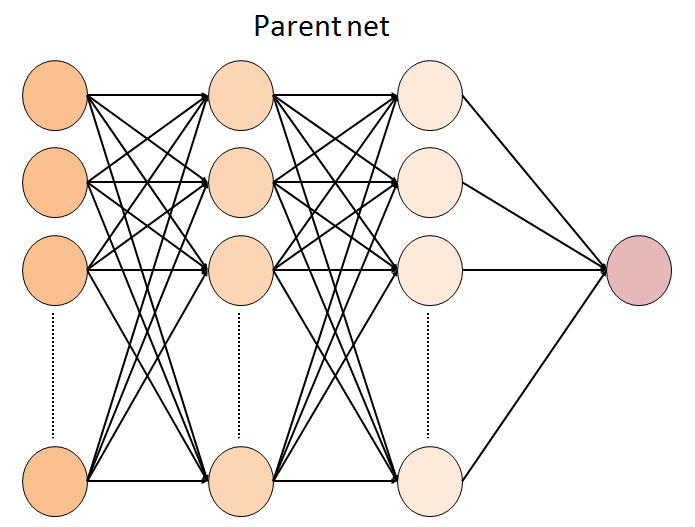
\includegraphics{plots/dropout.png}}
\end{figure}
\end{vbframe}

\begin{frame}{Dropout: Example}
\begin{figure}
\centering
\only<1>{\scalebox{0.8}{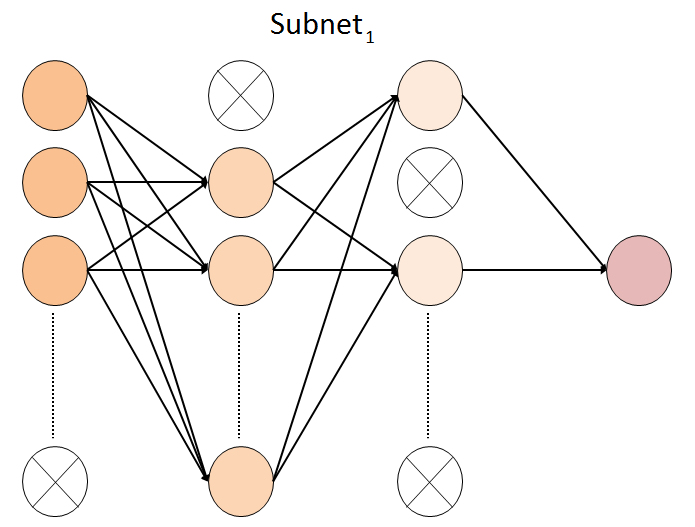
\includegraphics[width=10cm]{plots/subnet1.png}}}
\only<2>{\scalebox{0.8}{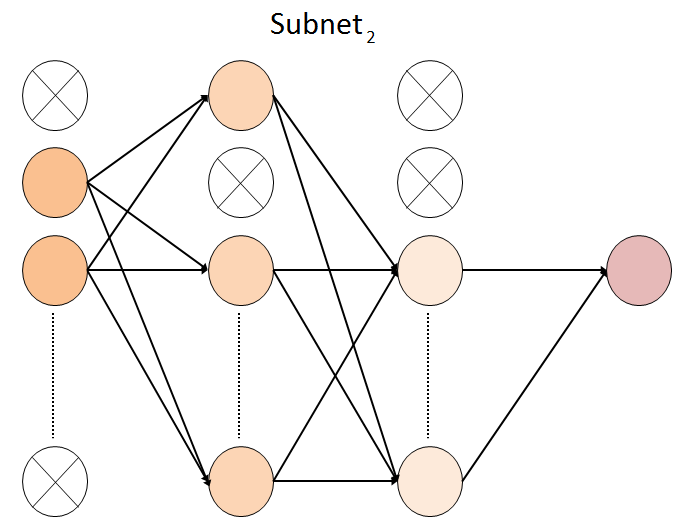
\includegraphics[width=10cm]{plots/subnet2.png}}}
\only<3>{\scalebox{0.8}{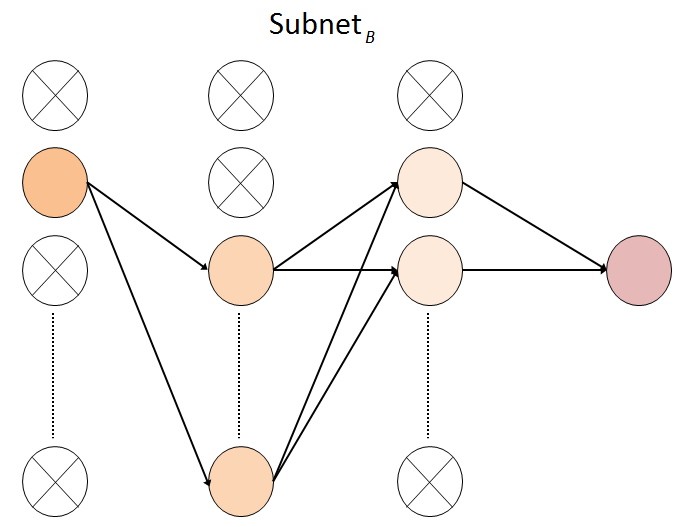
\includegraphics[width=10cm]{plots/subnet3.png}}}
\end{figure}
In each iteration, for each training example (in the forward pass), a different (random) subset of neurons is dropped out.
\end{frame}

%%%%%%%%%%%%%%%%%%%%%%%%%%%%%%%%%%%%%%%%%%%%5
\begin{vbframe}{Dropout: Algorithm}
\begin{itemize}
\item To train with dropout a minibatch-based learning algorithm such as stochastic gradient descent is used.  
\item For each training case in a minibatch, we randomly sample a binary vector/mask $\mu$ with one entry for each input or hidden unit in the network. The entries of $\mu$ are sampled independently from each other. 
\item The probability of sampling a mask value of 0 (dropout) for one unit is a hyperparameter known as the 'dropout rate'. 
\item A typical value for the dropout rate is $0.2$ for input units and $0.5$ for hidden units. 
\item Each unit in the network is multiplied by the corresponding mask value resulting in a $subnet_{\mu}$. 
\item Forward propagation, backpropagation, and the learning update are run as usual.

\framebreak


\begin{algorithm}[H]
\footnotesize
\caption{Training a (parent) neural network with dropout rate $p$}
\begin{algorithmic}[1]
\State Define parent network and initialize weights
\For{each minibatch: }
\For{each training sample: }
\State Draw mask $\mu$ using $p$
  \State Compute forward pass for $subnet_{\mu}$
  %        \State Compute the gradient of the loss for $network_{\mu}$
  \EndFor
\State \parbox[t]{\dimexpr\linewidth-\algorithmicindent}{Update the weights of the (parent) network by performing a gradient descent step with weight decay}
\EndFor
\end{algorithmic}
\end{algorithm}
\item The resulting derivatives for each parameter are averaged over the training cases in each mini-batch. Any training case which does not use a parameter contributes a gradient of zero for that parameter.
\end{itemize}
\end{vbframe}

\begin{vbframe}{Dropout: Weight scaling}
\begin{itemize}
\item The weights of the network will be larger than normal because of dropout. Therefore, to obtain a prediction at test time the weights must be first scaled by the chosen dropout rate.
\item This means that if a unit (neuron) is retrained with probability $p$ during training, the weight at test time of that unit is multiplied by $p$.
\begin{figure}
\centering
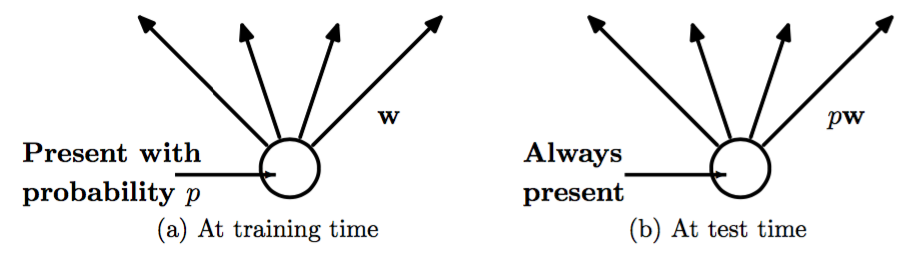
\includegraphics[width=7cm]{plots/dropout_neuron.png}
\tiny{\\ Credit: Srivastava et. al. (2014)}
\end{figure}
\item Rescaling of the weights can also be performed at training time instead, after each weight update at the end of the mini-batch. This is sometimes called 'inverse dropout'. Keras and PyTorch deep learning libraries implement dropout in this way.
% \item Weight scaling ensures that for any hidden unit the \textbf{expected} output (under the distribution used to drop units at training time) is the same as the \textbf{actual} output at test time. 
\end{itemize}
\end{vbframe}

%%%%%%%%%%%%%%%%%%%%%%%%%%%%%%%%%%%%%%%%%%%%%%%%%%%%%%%%%
\begin{vbframe}{Dropout: Example}
\begin{minipage}{0.5\textwidth}
\begin{itemize}
\item To demonstrate how dropout can easily improve generalization we compute neural networks with the structure showed on the right.
\item Each neural network we fit has different dropout probabilities, a tuple where one probability is for the input layer and one is for the hidden layers. We consider the tuples $(0;0) , (0.2;0.2) \text{ and } (0.6;0.5)$.
\end{itemize}
\end{minipage}
\begin{minipage}{0.45\textwidth}
\begin{figure}
\centering
\vspace{-0.5cm}
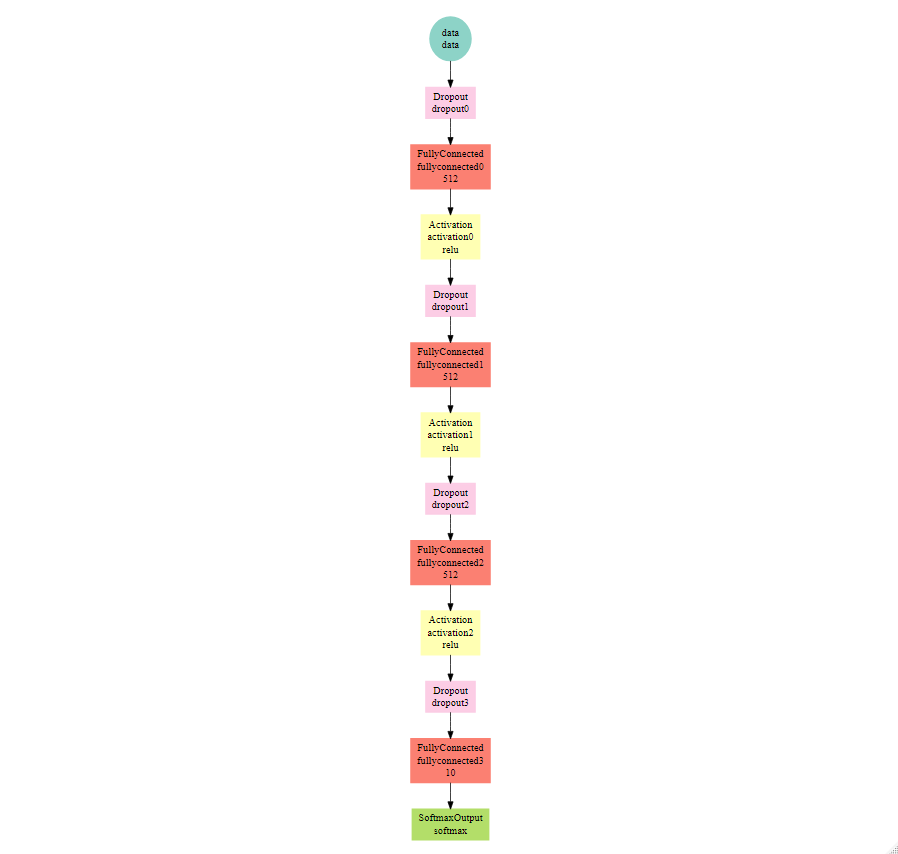
\includegraphics[width=9cm]{plots/mxnet_graph_dropout.png}
\end{figure}
\end{minipage}
\framebreak

\begin{center}
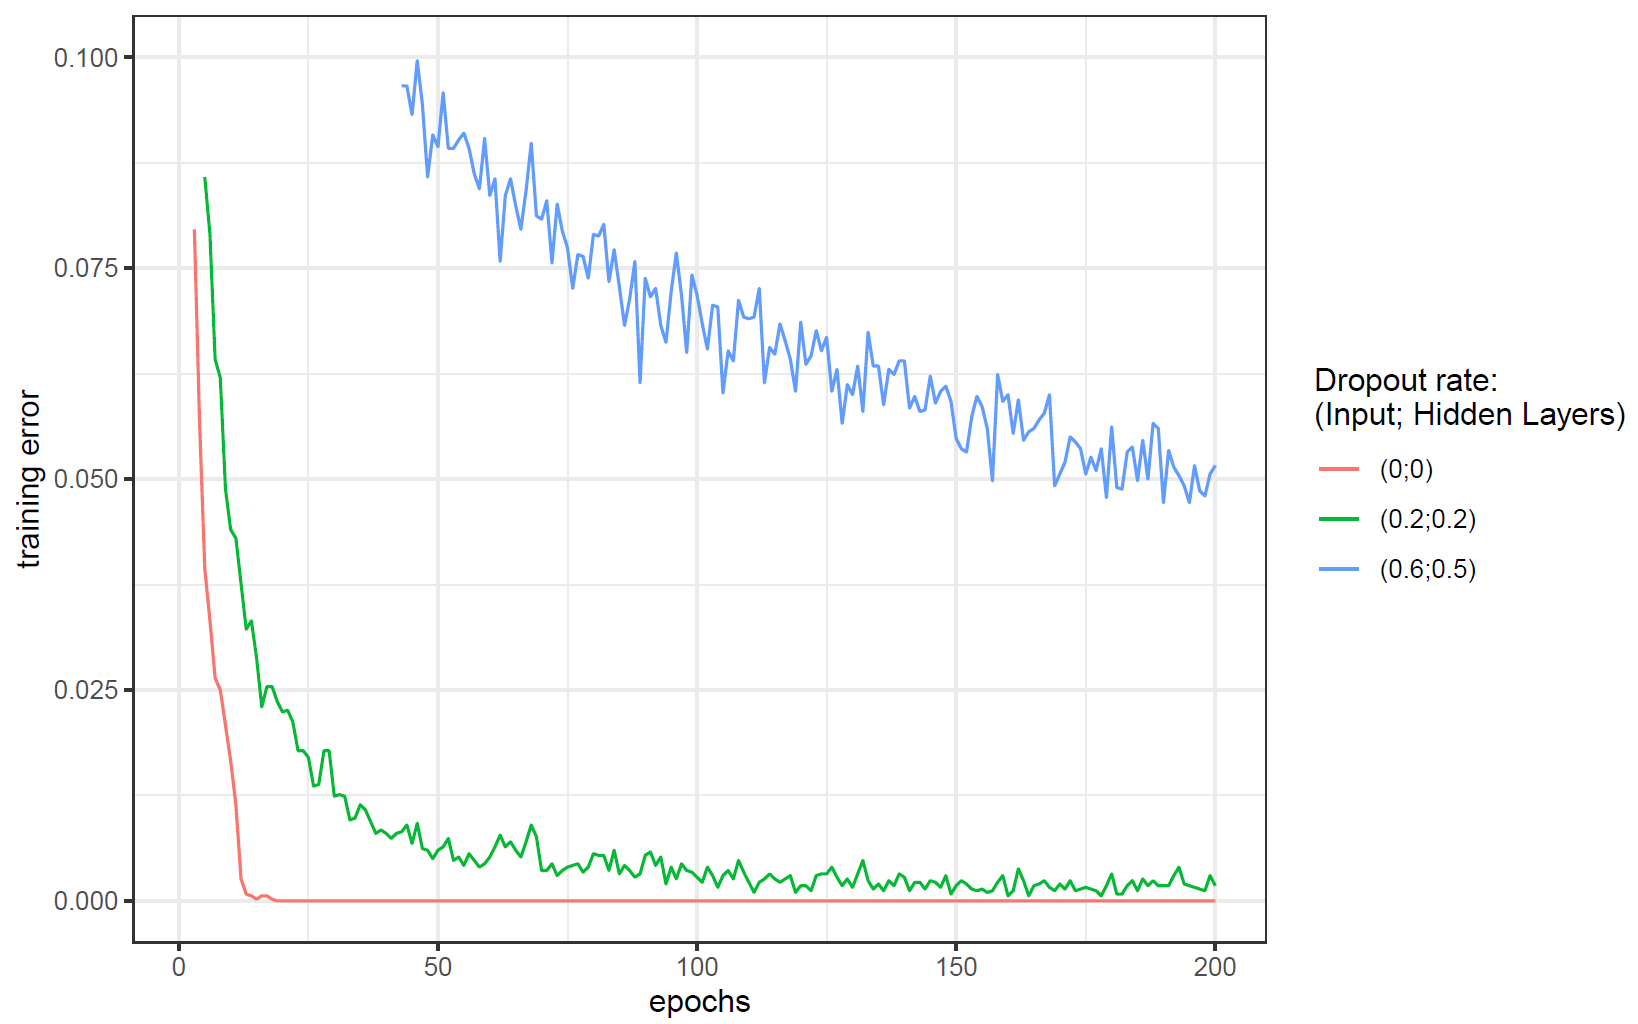
\includegraphics[width=0.9\textwidth]{plots/dropout01.png}
\end{center}

Higher dropout rates lead to higher training error. 
\framebreak

\begin{center}
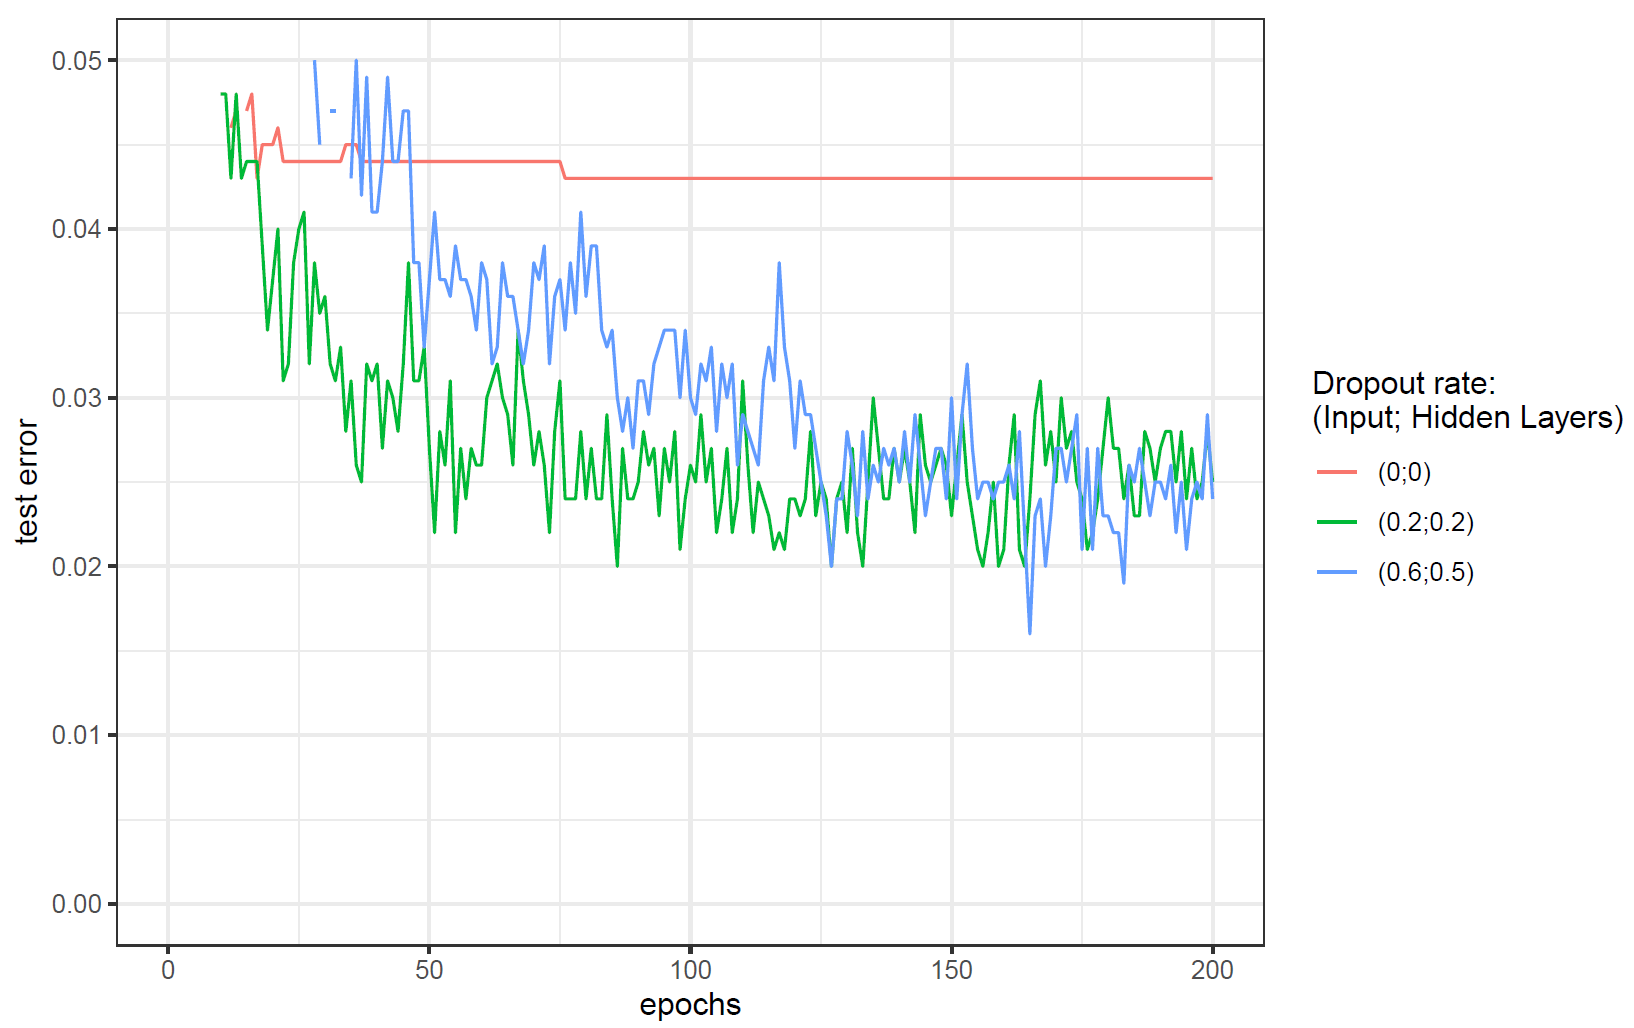
\includegraphics[width=0.9\textwidth]{plots/dropout02.png}
\end{center}

Dropout rate of 0 (no dropouts) leads to higher test error than dropping some units out. 
\end{vbframe}
%%%%%%%%%%%%%%%%%%%%%%%%%%%%%%%%%%%%%%%%%%%%%%%%%%%%%%%%%%%%%%%%%%
%%%%%%%%%%%%%%%%%%%%%%%%%%%%%%%%%%%%%%%%%%%%%%%%%%%%%%%%%%%%%%%%%%

\begin{vbframe}{Dropout, weight decay or both?}

\begin{center}
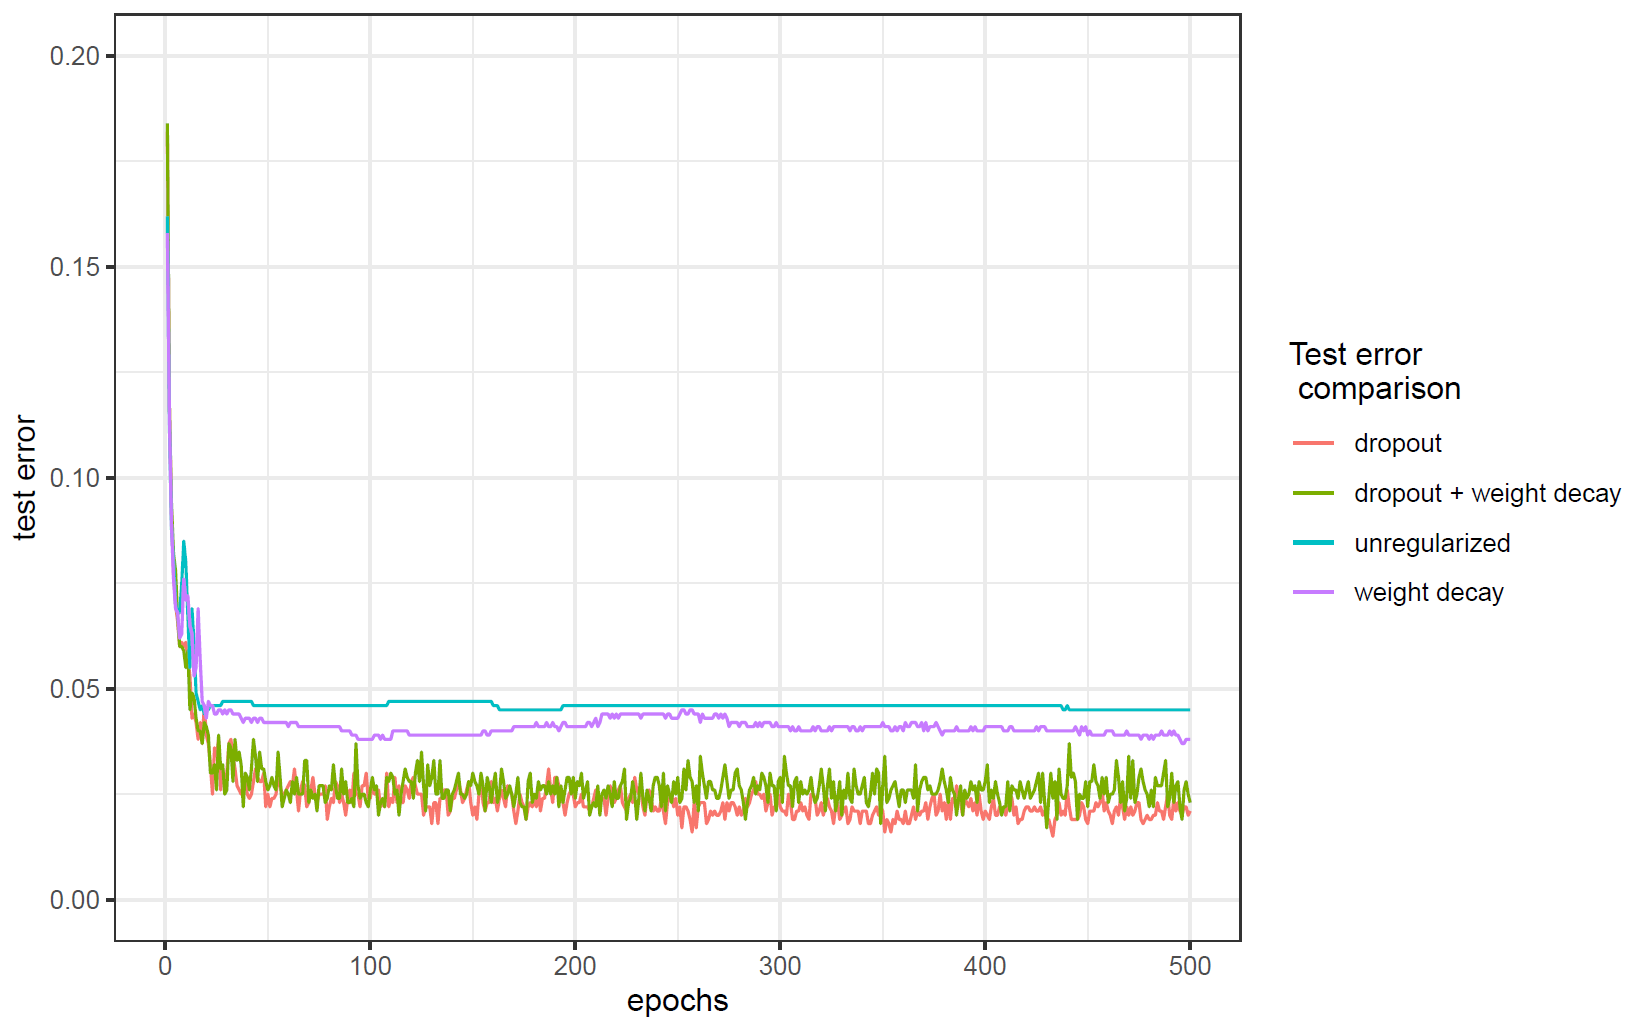
\includegraphics[width=0.9\textwidth]{plots/dropout03.png}
\end{center}

Here, dropout leads to a smaller test error than using no regularization or solely weight decay. 
\end{vbframe}

% %%%%%%%%%%%%%%%%%%%%%%%%%%%%%%%%%%%%%%%%%%%%%%%%%%%%%%%%%%%%%%%%%%
% \section{Dataset Augmentation}
% %%%%%%%%%%%%%%%%%%%%%%%%%%%%%%%%%%%%%%%%%%%%%%%%%%%%%%%%%%%%%%%%%%
% \begin{vbframe}{Dataset Augmentation}
%   \begin{itemize}
%     \item Problem: low generalization because high ratio of $$\frac{\text{complexity of the model}}{\text{\#train data}}$$
%     \item Idea: artificially increase the train data.
%       \begin{itemize}
%         \item Limited data supply $\rightarrow$ create \enquote{fake data}!
%       \end{itemize}
%     \item Increase variation in inputs \textbf{without} changing the labels.
%     \item Application:
%       \begin{itemize}
%         \item Image and Object recognition (rotation, scaling, pixel translation, flipping, noise injection, vignetting, color casting, lens distortion, injection of random negatives)
%         \item Speech recognition (speed augmentation, vocal tract perturbation)
%       \end{itemize}
%   \end{itemize}
% \framebreak
%   \begin{figure}
%     \centering
%       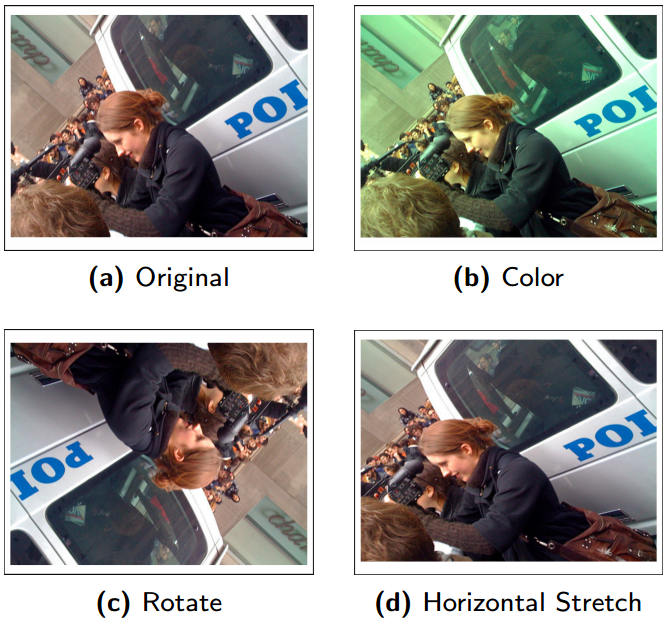
\includegraphics[width=7cm]{plots/data_augmentation_1.png}
%       \caption{(Wu et al. (2015))}
%   \end{figure}
% \framebreak
%   \begin{figure}
%     \centering
%       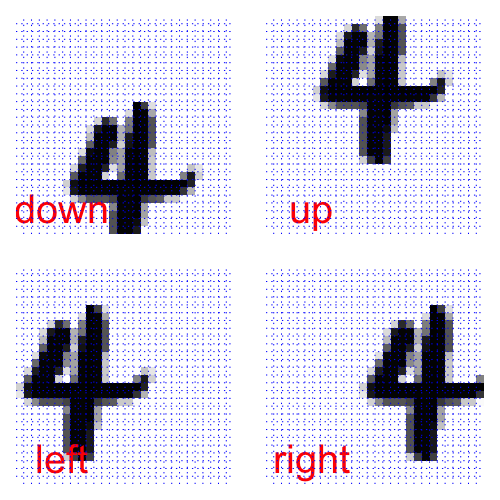
\includegraphics[width=6cm]{plots/data_augmentation_2.png}
%       \caption{(Wu et al. (2015))}
%   \end{figure}
%   $\Rightarrow$ Be careful when rotating digits (6 will become 9 and vice versa)!
% \end{vbframe}
% %%%%%%%%%%%%%%%%%%%%%%%%%%%%%%%%%%%%%%%%%%%%%%%%%%%%%%%%%%%%%%%%%%
% \section{Artifical Noise}
% %%%%%%%%%%%%%%%%%%%%%%%%%%%%%%%%%%%%%%%%%%%%%%%%%%%%%%%%%%%%%%%%%%
% \begin{vbframe}{Artificial Noise}
%   \begin{itemize}
%     \item Intentionally inject noise to the model, to make it more robust to small pertubations in the inputs.
%     \item This method may force the model to \enquote{grow} weights in regions of flat minima. Thus, the noisy model may not find perfect minima but its approximations lie in a flatter surrounding.
%     \item Bishop (1995) shows that the injection of artifical noise has the same effect as norm penalization strategies.
%     \item In practice, it is common to apply noise to the outputs. This strategy is termed label smoothing as it incorporates a small noise term on the labels of the classification outputs. The intuition is to account for possible errors in the labeling process.
%   \end{itemize}
% \end{vbframe}

%%%%%%%%%%%%%%%%%%%%%%%%%%%%%%%%%%%%%%%%%%%%%%%%%%%%%%%%%%%%%%%%%%
  %\section{References}
%%%%%%%%%%%%%%%%%%%%%%%%%%%%%%%%%%%%%%%%%%%%%%%%%%%%%%%%%%%%%%%%%%
  %%%%%%%%%%%%%%%%%%          REFERENCES          %%%%%%%%%%%%%%%%%%
  %%%%%%%%%%%%%%%%%%%%%%%%%%%%%%%%%%%%%%%%%%%%%%%%%%%%%%%%%%%%%%%%%%
  \begin{vbframe}
\frametitle{References}
\footnotesize{
  \begin{thebibliography}{99}
  %%%%%%%%%%%%%%%%%%%%%%%%%%%%%%%%%%
    \bibitem[Ian Goodfellow et al., 2016]{1} Ian Goodfellow, Yoshua Bengio and Aaron Courville (2016)
  \newblock Deep Learning
  \newblock \emph{\url{http://www.deeplearningbook.org/}}
  %%%%%%%%%%%%%%%%%%%%%%%%%%%%%%%%%%
    \bibitem[Hastie et al., 2009]{2} Trevor Hastie, Robert Tibshirani and Jerome Friedman (2009)
  \newblock The Elements of Statistical Learning
  \newblock \emph{\url{https://statweb.stanford.edu/\%7Etibs/ElemStatLearn/}}
  %%%%%%%%%%%%%%%%%%%%%%%%%%%%%%%%%%
    \bibitem[Hinton et al., 2012]{3} Geoffrey E Hinton, Nitish Srivastava, Alex Krizhevsky Ilya Sutskever and Ruslan Salakhutdinov (2012)
  \newblock Improving neural networks by preventing co-adaptation of feature detectors
  \newblock \emph{\url{http://arxiv.org/abs/1207.0580}}
  %%%%%%%%%%%%%%%%%%%%%%%%%%%%%%%%%%
    \bibitem[Srivastava et. al., 2014]{4} Nitish Srivastava, Geoffrey Hinton, Alex Krizhevsky Ilya Sutskever and Ruslan Salakhutdinov (2012)
  \newblock Dropout:  A Simple Way to Prevent Neural Networks from Overfitting
  \newblock Journal of Machine Learning Research 15 (2014) 1929-1958
  \newblock \emph{\url{http://jmlr.org/papers/v15/srivastava14a.html}}
  %%%%%%%%%%%%%%%%%%%%%%%%%%%%%%%%%%
    \bibitem[Brownlee, 2018]{5} Jason Brownlee (2018) 
  \newblock A Gentle Introduction to Dropout for Regularizing Deep Neural Networks
  \newblock \emph{\url{https://machinelearningmastery.com/dropout-for-regularizing-deep-neural-networks/}}
%   %%%%%%%%%%%%%%%%%%%%%%%%%%%%%%%%%%
% \bibitem[Wu et al., 2015]{4} Wu Ren, Yan Shengen, Shan Yi, Dang Qingqing and Sun Gang (2015)
% \newblock Deep Image: Scaling up Image Recognition
% \newblock \emph{\url{https://arxiv.org/abs/1501.02876}}
%   %%%%%%%%%%%%%%%%%%%%%%%%%%%%%%%%%%
% \bibitem[Bishop, Chris M., 1995]{5} Bishop, Chris M. (1995)
% \newblock Training with Noise is Equivalent to Tikhonov Regularization
% \newblock \emph{\url{https://www.microsoft.com/en-us/research/wp-content/uploads/2016/02/bishop-tikhonov-nc-95.pdf}}

  \end{thebibliography}
}
\end{vbframe}

\endlecture
\end{document}